\chapter{Molecole}

Definiamo le grandezze in gioco per un sistema molecolare:
\begin{itemize}
    \item \( N_N \): numero totale di nuclei
    \item \( Z_k \): numero atomico del \( k \)-esimo nucleo (con \( k=1, \dots, N_N \))
    \item \( M_k \): massa del \( k \)-esimo nucleo
    \item \( N_e \): numero totale di elettroni
\end{itemize}

L'Hamiltoniana completa del sistema molecolare si scrive come somma delle energie cinetiche e potenziali di tutte le particelle:
\begin{align}
    H &= \underbrace{\sum_{i=1}^{N_e} -\frac{\hbar^2}{2m_e} \nabla_{\vec{r}_i}^2}_{T_e} 
    + \underbrace{\sum_{i=1}^{N_e} \sum_{k=1}^{N_N} -\frac{Z_k e^2}{4\pi\varepsilon_0 |\vec{r}_i - \vec{R}_k|}}_{V_{Ne}} 
    + \underbrace{\frac{1}{2} \sum_{\substack{i,j \\ i \neq j}}^{N_e} \frac{e^2}{4\pi\varepsilon_0 r_{ij}}}_{V_{ee}} \nonumber \\[1.5ex]
    &\quad + \underbrace{\frac{1}{2} \sum_{\substack{k,\ell \\ k \neq \ell}}^{N_N} \frac{Z_k Z_\ell e^2}{4\pi\varepsilon_0 |\vec{R}_k - \vec{R}_\ell|}}_{V_{NN}} 
    + \underbrace{\sum_{k=1}^{N_N} -\frac{\hbar^2}{2M_k} \nabla_{\vec{R}_k}^2}_{T_N} 
    + \Delta H_{\text{correz.}}
\end{align}

Ovvero, in forma più compatta:
\begin{equation}
    H \simeq T_e + V_{Ne} + V_{ee} + T_N + V_{NN}
\end{equation}

\begin{attention}
    L'Hamiltoniana \( H \) è scritta nel sistema di riferimento del laboratorio (\textbf{SR LAB}, fisso). \\
    Le distanze relative sono definite vettorialmente come:
    \begin{align}
        \vec{r}_{ij} &= \vec{r}_j - \vec{r}_i = \vec{r}_{e,j} - \vec{r}_{e,i} \\
        \vec{R}_{k\ell} &= \vec{R}_k - \vec{R}_\ell
    \end{align}
\end{attention}

La funzione d'onda completa del sistema dipende da tutte le coordinate spaziali e di spin degli elettroni, nonché dalle coordinate spaziali dei nuclei:
\begin{equation}
    \Psi_E(\vec{r}_1, \dots, \vec{r}_{N_e}, \vec{s}_1, \dots, \vec{s}_{N_e}, \vec{R}_1, \dots, \vec{R}_{N_N})
\end{equation}

Per semplificare la notazione, introduciamo le coordinate generalizzate per gli elettroni \( \tilde{q}_i = (\vec{r}_i, \vec{s}_i) \) e raggruppiamo l'insieme delle coordinate nucleari in \( \tilde{R}_{N_N} = (\vec{R}_1, \dots, \vec{R}_{N_N}) \).

Gli elettroni, avendo una massa molto inferiore a quella dei nuclei, possiedono una dinamica molto più veloce. Di conseguenza, in prima approssimazione si può pensare di \textbf{considerare i nuclei fermi} rispetto al moto elettronico. 

Sotto questa ipotesi, la funzione d'onda totale del sistema si può fattorizzare nel prodotto di due contributi:
\begin{equation}
    \Psi_E \simeq \underbrace{\Psi_{E,e}(\tilde{q}_1, \dots, \tilde{q}_{N_e} ; \tilde{R}_{N_N})}_{\substack{\text{parte elettronica} \\ \text{(dipende parametricamente} \\ \text{dai nuclei fissi)}}} \cdot \underbrace{\Psi_{E,N}(\tilde{R}_{N_N})}_{\text{parte nucleare}}
\end{equation}

Risolviamo prima la parte elettronica e poi quella nucleare, ricordando di considerare la parte elettronica all'interno di quella nucleare.

\begin{itemize}
    \item \textbf{Problema elettronico}: trascurando \(\Delta H_{\text{correz.}}\), si risolve l'equazione mantenendo le coordinate nucleari \(\tilde{R}_{N_N}\) come \textbf{parametri fissi}:
    \begin{equation}
        (T_e + V_{Ne} + V_{ee}) \Psi_{E,e}(\tilde{q}_1, \dots, \tilde{q}_{N_e} ; \tilde{R}_{N_N}) = E_e \Psi_{E,e}(\tilde{q}_1, \dots, \tilde{q}_{N_e} ; \tilde{R}_{N_N})
    \end{equation}

    \item \textbf{Problema nucleare}: il termine \(E_e(\tilde{R}_{N_N})\), che dipendeva dai parametri fissati nello step precedente, funge ora da energia potenziale per l'Hamiltoniana nucleare:
    \begin{equation}
        H_N = T_N + V_{NN} + E_e(\tilde{R}_{N_N})
    \end{equation}
    \begin{equation}
        H_N \Psi_{E,N}(\tilde{R}_{N_N}) = E_N \Psi_{E,N}(\tilde{R}_{N_N})
    \end{equation}

    \item \textbf{Energia totale}: l'energia complessiva del sistema è semplicemente la somma:
    \begin{equation}
        E_{\text{TOT}} = E_N + E_e
    \end{equation}
\end{itemize}

\begin{remark}
    Consideriamo l'effetto degli \(e^-\) come energia potenziale media: il loro contributo è mediato ma tiene conto della distanza spaziale che hanno tra loro (che non sono uguali). Più siamo precisi nel definirla, più avremo una \(\Psi\) precisa.
\end{remark}


\section{Parte elettronica}

\lezione{12}{31/03/2026}

La soluzione del problema elettronico parte dall'approssimazione dell'Hamiltoniana. Trascurando ulteriori correzioni, si ottiene:
\begin{equation}
    H_e \simeq T_e + \underbrace{V_{e-N}}_{\text{nucleo}} + V_{ee}
\end{equation}

Dato che le coordinate nucleari \(\tilde{R}_{N_N}\) sono trattate come parametri fissi, d'ora in poi omettiamo di scriverle esplicitamente per alleggerire la notazione:
\begin{equation}
    \Psi_{E,e}(\tilde{r}_{N_e}, \tilde{s}_{N_e} ; \underbrace{\tilde{R}_{N_N}}_{\text{fissa (parametri)}}) \longrightarrow \Psi_{E,e}(\tilde{r}_{N_e}, \tilde{s}_{N_e})
\end{equation}

Procediamo applicando la separazione delle variabili tra la parte spaziale e la parte di spin della funzione d'onda elettronica:
\begin{equation}
    \Psi_{E,e}(\tilde{r}_{N_e}, \tilde{s}_{N_e}) = \Psi_{E,e}(\tilde{r}_{N_e}) \underbrace{\chi(\tilde{s}_{N_e})}_{\text{separazione variabili}}
\end{equation}

Approfondiremo quindi la soluzione dell'equazione agli autovalori limitandoci esclusivamente alla componente spaziale:
\begin{equation}
    H_e \Psi_{E,e}(\tilde{r}_{N_e}) = \underbrace{E_e(\tilde{R}_{N_N})}_{\text{fissi (param.)}} \Psi_{E,e}(\tilde{r}_{N_e})
\end{equation}

Usiamo il metodo \textbf{LCAO} (Linear Combination of Atomic Orbitals).
È un metodo approssimato per lo studio delle molecole che prevede le seguenti ipotesi:

\begin{enumerate}
    \item \textbf{Interazione nucleo-nucleo trascurabile} (\( V_{NN} \)): riteniamo i nuclei sufficientemente lontani affinché si possano separare le variabili (il contributo dell'interazione nucleare verrà aggiunto in un secondo momento).
    
    \item \textbf{I nuclei sono fissi}.
    
    \item \textbf{Combinazione lineare}: la funzione d'onda elettronica viene approssimata come:
    \begin{equation}
        \Psi_{E,e}(\tilde{r}_{N_e}) \simeq \sum_k c_k \varphi_{E,k}
    \end{equation}
    Questa espressione rappresenta una combinazione lineare di autofunzioni di singola particella (\(\varphi_{E,k}\)), ovvero una \textbf{combinazione di orbitali atomici}. Il sistema globale viene descritto tramite tanti sottosistemi, ciascuno caratterizzato da un elettrone che interagisce con un nucleo.
\end{enumerate}

Tale soluzione approssimata la indicheremo con \(\Psi_{E, \text{LCAO}}\).

\subsubsection{Idrogeno ionizzato}
Applicazione del metodo ad una molecola \( H_2^+ \) (idrogeno ionizzato). \\
La molecola \( H_2^+ \) risulta comoda per il calcolo poiché:
\begin{enumerate}
    \item \( V_{ee} = 0 \) (essendo presente un solo elettrone).
    \item L'Hamiltoniana elettronica assume la forma:
    \begin{equation}
        H_e = -\frac{\hbar^2}{2m_e} \nabla_{\vec{r}}^2 - \frac{Z_A e^2}{4\pi\varepsilon_0 r_A} - \frac{Z_B e^2}{4\pi\varepsilon_0 r_B}
    \end{equation}
\end{enumerate}

\begin{figure}[htbp]
    \centering
    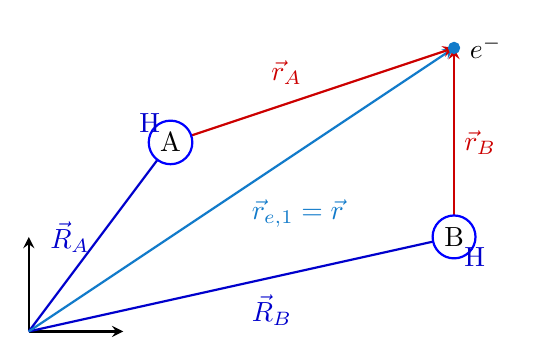
\begin{tikzpicture}[>=stealth, thick, scale=1.2]
        % Origine
        \coordinate (O) at (0,0);
        
        % Posizioni Nuclei ed Elettrone
        \coordinate (A) at (1.5, 2);
        \coordinate (B) at (4.5, 1);
        \coordinate (E) at (4.5, 3);

        % Assi di riferimento cartesiani
        \draw[->] (O) -- (1,0);
        \draw[->] (O) -- (0,1);
        
        % Vettori posizione dal SR (nuclei)
        \draw[->, blue!80!black] (O) -- (A) node[midway, left] {\( \vec{R}_A \)};
        \draw[->, blue!80!black] (O) -- (B) node[midway, below right] {\( \vec{R}_B \)};
        
        % Vettore posizione elettrone dal SR
        \draw[->, cyan!60!blue] (O) -- (E) node[midway, below right] {\( \vec{r}_{e,1} = \vec{r} \)};

        % Vettori distanza relativa elettrone-nucleo
        \draw[->, red!80!black] (A) -- (E) node[midway, above left] {\( \vec{r}_A \)};
        \draw[->, red!80!black] (B) -- (E) node[midway, right] {\( \vec{r}_B \)};

        % Nodi grafici (Nuclei ed Elettrone)
        \node[circle, draw=blue, fill=white, inner sep=2pt] (nodeA) at (A) {A};
        \node[above left, blue!80!black] at (nodeA) {H};
        
        \node[circle, draw=blue, fill=white, inner sep=2pt] (nodeB) at (B) {B};
        \node[below right, blue!80!black] at (nodeB) {H};
        
        \filldraw[cyan!60!blue] (E) circle (1.5pt) node[right=2pt, text=black] {\( e^- \)};

    \end{tikzpicture}
    \caption{Coordinate vettoriali per la molecola \( H_2^+ \).}
    \label{fig:coordinate_h2_plus}
\end{figure}

\begin{remark}
    Date le chiusure vettoriali nel grafico, vale la relazione: \( \vec{r} = \vec{r}_A + \vec{R}_A = \vec{r}_B + \vec{R}_B \).
\end{remark}

Definiamo le Hamiltoniane imperturbate per i singoli atomi isolati:
\begin{align}
    H_A^{(0)} &= -\frac{\hbar^2}{2m_e} \nabla_{\vec{r}}^2 - \frac{Z_A e^2}{4\pi\varepsilon_0 r_A} \\[1.5ex]
    H_B^{(0)} &= -\frac{\hbar^2}{2m_e} \nabla_{\vec{r}}^2 - \frac{Z_B e^2}{4\pi\varepsilon_0 r_B}
\end{align}

Le relative equazioni agli autovalori sono:
\begin{equation}
    H_A^{(0)} \varphi_A^{(0)} = E_A^{(0)} \varphi_A^{(0)} \qquad \qquad H_B^{(0)} \varphi_B^{(0)} = E_B^{(0)} \varphi_B^{(0)}
\end{equation}

Nella molecola monoelementale (\( H_2^+ \)):
\begin{equation}
    Z_A = Z_B = 1 \implies E_A^{(0)} = E_B^{(0)} = E^{(0)}
\end{equation}

Procediamo applicando l'Hamiltoniana elettronica complessiva \( H_e \) alla funzione d'onda approssimata tramite combinazione lineare (\( \Psi_{e,LCAO} \)):

\begin{align}
    H_e \Psi_{e,LCAO} &= \left( -\frac{\hbar^2}{2m_e} \nabla_{\vec{r}}^2 - \frac{Z_A e^2}{4\pi\varepsilon_0 r_A} - \frac{Z_B e^2}{4\pi\varepsilon_0 r_B} \right) \underbrace{\left( c_A \varphi_A^{(0)} + c_B \varphi_B^{(0)} \right)}_{\Psi_{e,LCAO}} = \nonumber \\[2ex]
    &= c_A E_A^{(0)} \varphi_A^{(0)} + c_A \left( -\frac{Z_B e^2}{4\pi\varepsilon_0 r_B} \right) \varphi_A^{(0)} + c_B E_B^{(0)} \varphi_B^{(0)} + c_B \left( -\frac{Z_A e^2}{4\pi\varepsilon_0 r_A} \right) \varphi_B^{(0)}
\end{align}

Imponendo l'equazione di Schrödinger \( H_e \Psi_{e,LCAO} = E_{LCAO} \Psi_{e,LCAO} \), la quantità calcolata deve eguagliare:
\begin{equation}
    = E_{LCAO} \underbrace{\left( c_A \varphi_A^{(0)} + c_B \varphi_B^{(0)} \right)}_{\Psi_{e,LCAO}}
\end{equation}

Usiamo l'ipotesi \( E_A^{(0)} = E_B^{(0)} = E^{(0)} \) (molecola monoelementale) e poi portiamo al primo membro, esplicitando i coefficienti \( c_A, c_B \) che non sono noti:
\begin{equation}
    c_A \left[ E^{(0)} - \frac{Z_B e^2}{4\pi\varepsilon_0 r_B} - E_{LCAO} \right] \varphi_A^{(0)} + c_B \left[ E^{(0)} - \frac{Z_A e^2}{4\pi\varepsilon_0 r_A} - E_{LCAO} \right] \varphi_B^{(0)} = 0
\end{equation}

Definiamo la variazione di energia:
\begin{equation}
    \Delta E := E_{LCAO} - E^{(0)}
\end{equation}

Sostituendo la definizione di \( \Delta E \) otteniamo:
\begin{equation}
    \implies c_A \left[ -\Delta E - \frac{Z_B e^2}{4\pi\varepsilon_0 r_B} \right] \varphi_A^{(0)} + c_B \left[ -\Delta E - \frac{Z_A e^2}{4\pi\varepsilon_0 r_A} \right] \varphi_B^{(0)} = 0
\end{equation}

Proiettiamo l'equazione sugli stati \( \bra{\varphi_A^{(0)}} \) e \( \bra{\varphi_B^{(0)}} \), ottenendo il seguente sistema di equazioni:
\begin{align}
    \bra{\varphi_A^{(0)}} c_A \left[ -\Delta E - \frac{Z_B e^2}{4\pi\varepsilon_0 r_B} \right] \ket{\varphi_A^{(0)}} + \bra{\varphi_A^{(0)}} c_B \left[ -\Delta E - \frac{Z_A e^2}{4\pi\varepsilon_0 r_A} \right] \ket{\varphi_B^{(0)}} &= 0 \\[1.5ex]
    \bra{\varphi_B^{(0)}} c_A \left[ -\Delta E - \frac{Z_B e^2}{4\pi\varepsilon_0 r_B} \right] \ket{\varphi_A^{(0)}} + \bra{\varphi_B^{(0)}} c_B \left[ -\Delta E - \frac{Z_A e^2}{4\pi\varepsilon_0 r_A} \right] \ket{\varphi_B^{(0)}} &= 0
\end{align}

Le uniche incognite del sistema sono i coefficienti \( c_A, c_B \). 
Analizziamo i vari termini che emergono dalle proiezioni:
\begin{itemize}
    \item \textbf{Normalizzazione}:
    \begin{equation}
        \braket{\varphi_A^{(0)}}{\varphi_A^{(0)}} = 1
    \end{equation}
    
    \item \textbf{Integrale di Coulomb} (\( C_1 \)):
    \begin{equation}
        \mel{\varphi_A^{(0)}}{-\frac{Z_B e^2}{4\pi\varepsilon_0 r_B}}{\varphi_A^{(0)}} = C_1
    \end{equation}
    
    \item \textbf{Integrale di sovrapposizione} (\( S \)):
    \begin{equation}
        \braket{\varphi_A^{(0)}}{\varphi_B^{(0)}} = S
    \end{equation}
    
    \item \textbf{Integrale di scambio o di risonanza} (\( D_1 \)):
    \begin{equation}
        \mel{\varphi_A^{(0)}}{-\frac{Z_A e^2}{4\pi\varepsilon_0 r_A}}{\varphi_B^{(0)}} = D_1
    \end{equation}
\end{itemize}

Proiettando rispetto a \( \ket{\varphi_B^{(0)}} \) si ottengono gli stessi termini analoghi (\( C_2, D_2 \)).

Se la molecola è monoelementale (omonucleare), per ragioni di simmetria gli integrali relativi ai due nuclei risultano uguali: \( C_1 = C_2 = C \) e \( D_1 = D_2 = D \). % [Testo originale indica "monoatomica", ma il termine corretto è monoelementale/omonucleare]

Sostituendo queste definizioni, il problema si riduce al seguente sistema lineare omogeneo:
\begin{equation}
    \implies \text{sistema} \quad
    \begin{cases}
        (C_1 - \Delta E) c_A + (D_1 - \Delta E \cdot S) c_B = 0 \\[1.5ex]
        (D_2 - \Delta E \cdot S) c_A + (C_2 - \Delta E) c_B = 0
    \end{cases}
\end{equation}

Le funzioni d'onda di singola particella hanno in generale la forma:
\begin{align}
    \varphi_A^{(0)} &\longrightarrow R_{n_A \ell_A}(r) Y_{\ell_A}^{m_{\ell_A}}(\theta, \phi) \\[1.5ex]
    \varphi_B^{(0)} &\longrightarrow R_{n_B \ell_B}(r) Y_{\ell_B}^{m_{\ell_B}}(\theta, \phi)
\end{align}

Nello stato fondamentale si ha:
\begin{equation}
    \varphi_A^{(0)} = \varphi_B^{(0)} = R_{10} Y_0^0
\end{equation}
con energie coincidenti:
\begin{equation}
    E_A^{(0)} = E_B^{(0)} = E^{(0)}
\end{equation}

\begin{remark}
    Questa relazione di uguaglianza vale in generale quando gli stati sono identici, non esclusivamente per lo stato fondamentale.
\end{remark}

In questa ipotesi (\( E_A^{(0)} = E_B^{(0)} = E^{(0)} \)) e per atomi identici (\( A=B \), come per la molecola di idrogeno con \( Z_A = Z_B \)), gli integrali si semplificano:
\begin{equation}
    C_1 = C_2 = C \qquad D_1 = D_2 = D
\end{equation}

Il sistema di equazioni si riduce pertanto a:
\begin{equation}
    \begin{cases}
        (C - \Delta E) c_A + (D - \Delta E \cdot S) c_B = 0 \\[1.5ex]
        (D - \Delta E \cdot S) c_A + (C - \Delta E) c_B = 0
    \end{cases}
\end{equation}

Affinché il sistema ammetta soluzioni non banali, il determinante dei coefficienti deve annullarsi:
\begin{equation}
    (C - \Delta E)^2 - (D - S \cdot \Delta E)^2 = 0
\end{equation}

L'equazione ha due soluzioni, che corrispondono alla condizione sui coefficienti \( c_A = \pm c_B \):
\begin{equation}
    \Delta E_+ = \frac{C + D}{1 + S} \qquad \Delta E_- = \frac{C - D}{1 - S}
\end{equation}

Spesso queste soluzioni vengono espresse in modo sintetico come:
\begin{equation}
    \Delta E_{\pm} = \frac{C \pm D}{1 \pm S}
\end{equation}

Poiché \( \Delta E_+ < \Delta E_- \), si osserva una rimozione della degenerazione dato che i due valori sono diversi.
Ricordiamo la definizione della variazione di energia:
\begin{equation}
    \Delta E = E_{\text{LCAO}} - E^{(0)}
\end{equation}

Quando la distanza internucleare \( R_{AB} \to \infty \), gli atomi sono isolati e ciascuno possiede il proprio livello energetico imperturbato \( E^{(0)} \). Quando gli atomi si avvicinano, l'interazione provoca uno splitting dei livelli.

\begin{figure}[htbp]
    \centering
    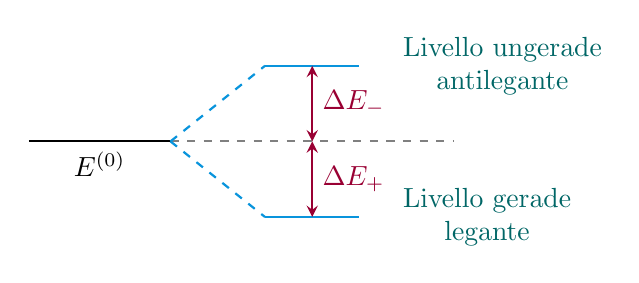
\begin{tikzpicture}[>=stealth, thick, scale=1.2, every node/.style={align=center}]
        
        % Livelli isolati
        \draw (-2.5, 0) -- (-1, 0) node[midway, below] {\( E^{(0)} \)};
        
        % Linea di riferimento centrale
        \draw[dashed, gray] (-1, 0) -- (2, 0);
        
        % Livelli splittati
        \draw[cyan!80!blue] (0, 0.8) -- (1, 0.8) node[right, xshift = 12pt, teal!80!black] {Livello ungerade \\ antilegante};
        \draw[cyan!80!blue] (0, -0.8) -- (1, -0.8) node[ right, xshift = 12pt, teal!80!black] {Livello gerade \\ legante};
        
        % Linee di collegamento
        \draw[dashed, cyan!80!blue] (-1, 0) -- (0, 0.8);
        \draw[dashed, cyan!80!blue] (-1, 0) -- (0, -0.8);
        
        % Frecce Delta E
        \draw[<->, purple!80!black] (0.5, 0) -- (0.5, 0.8) node[midway, right] {\( \Delta E_- \)};
        \draw[<->, purple!80!black] (0.5, 0) -- (0.5, -0.8) node[midway, right] {\( \Delta E_+ \)};
        
        
    \end{tikzpicture}
    \caption{Splitting dei livelli energetici all'avvicinarsi degli atomi.}
    \label{fig:splitting_lcao}
\end{figure}

Mantenendo i nuclei fissi (ovvero fissati i vettori posizione \( \vec{R}_A, \vec{R}_B \)), l'energia del sistema in funzione della distanza internucleare \( R_{AB} \) è data da \( E_{\text{LCAO}} \), da cui si valuta \( \Delta E = E_{\text{LCAO}} - E^{(0)} \).

\begin{figure}[htbp]
    \centering
    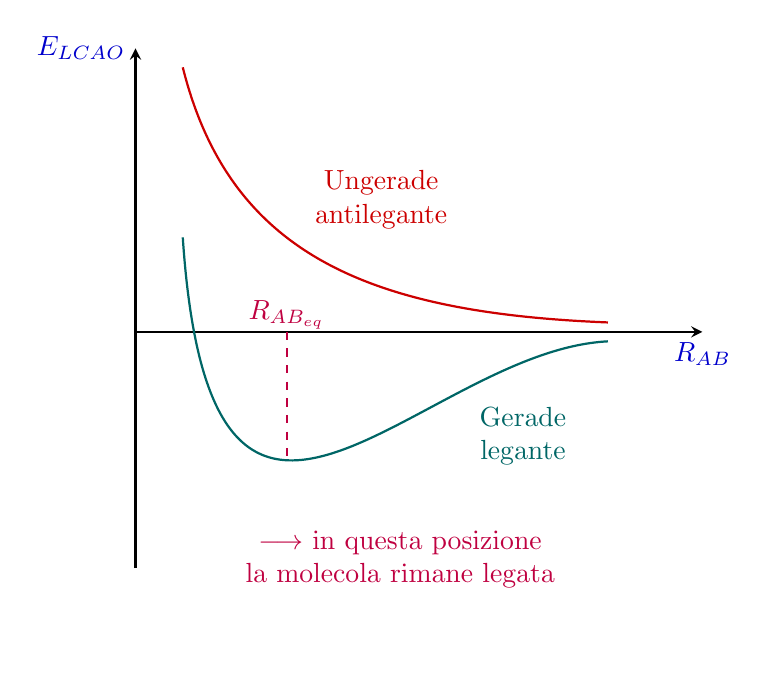
\begin{tikzpicture}[>=stealth, thick, scale=1.2]
        
        % Assi
        \draw[->] (0, -2.5) -- (0, 3) node[left, blue!80!black] {\( E_{\text{LCAO}} \)};
        \draw[->] (0, 0) -- (6, 0) node[below, blue!80!black] {\( R_{AB} \)};
        
        % Curva Ungerade (Antilegante)
        \draw[red!80!black] (0.5, 2.8) .. controls (1, 0.8) and (2.5, 0.2) .. (5, 0.1);
        \node[red!80!black, align=center] at (2.6, 1.4) {Ungerade \\ antilegante};
        
        % Curva Gerade (Legante)
        \draw[teal!80!black] (0.5, 1) .. controls (0.8, -3.5) and (3, -0.2) .. (5, -0.1);
        \node[teal!80!black, align=center] at (4.1, -1.1) {Gerade \\ legante};
        
        % Posizione di equilibrio
        \draw[dashed, purple] (1.6, 0) -- (1.6, -1.4) node[above, yshift = 45pt] {\( R_{AB_{eq}} \)};
        
        \node[purple, align=center, below] at (2.8, -2.0) {\(\longrightarrow\) in questa posizione \\ la molecola rimane legata};
        
    \end{tikzpicture}
    \caption{Curve dell'energia potenziale \( E_{\text{LCAO}} \) in funzione della distanza internucleare \( R_{AB} \).}
    \label{fig:curve_energia_lcao}
\end{figure}


Dalle soluzioni ricavate per i coefficienti, possiamo distinguere due casi principali per la funzione d'onda molecolare \(\Psi_{E, \text{LCAO}}\):

\begin{itemize}
    \item Se \( c_A = c_B \), otteniamo la soluzione simmetrica detta \textbf{gerade} (pari):
    \begin{equation}
        \Psi_{E, \text{LCAO}} = c_A \varphi_A^{(0)} + c_A \varphi_B^{(0)} = \Psi_{+, G} \quad \text{gerade}
    \end{equation}
    
    \item Se \( c_A = -c_B \), otteniamo la soluzione antisimmetrica detta \textbf{ungerade} (dispari):
    \begin{equation}
        \Psi_{E, \text{LCAO}} = c_A \varphi_A^{(0)} - c_A \varphi_B^{(0)} = \Psi_{-, U} \quad \text{ungerade}
    \end{equation}
\end{itemize}

Gli andamenti delle funzioni d'onda e delle relative densità di probabilità rispetto alle posizioni dei nuclei (A e B) evidenziano la natura legante o antilegante dei due stati.

\begin{figure}[htbp]
    \centering
    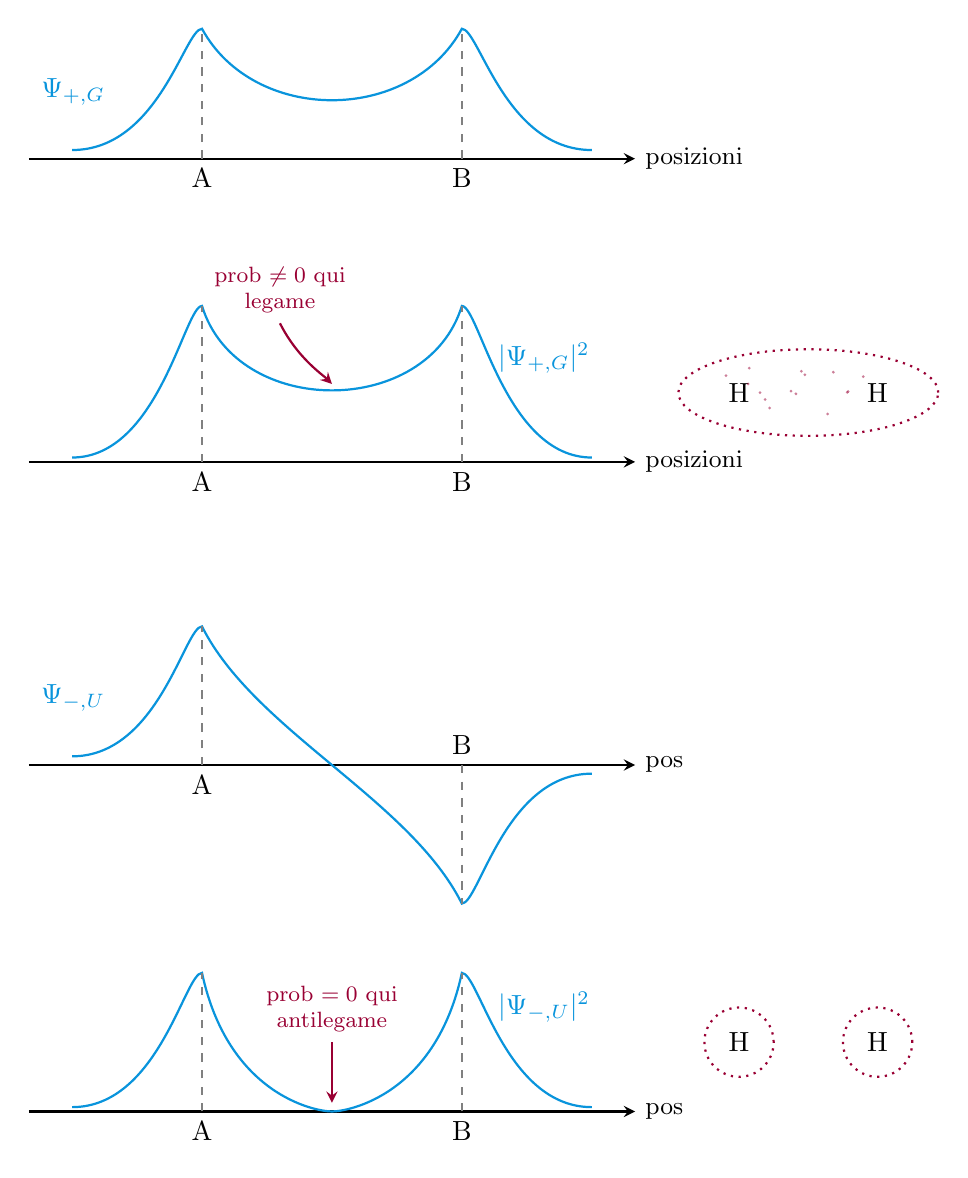
\begin{tikzpicture}[>=stealth, thick, scale=1.1]
        
        % Definizioni posizioni nuclei
        \def\xA{-1.5}
        \def\xB{1.5}
        
        % ----------------------------------------------------
        % 1. Funzione d'onda Gerade \Psi_{+, G}
        % ----------------------------------------------------
        \begin{scope}[yshift=7cm]
            \draw[->] (-3.5, 0) -- (3.5, 0) node[right, font=\small] {posizioni};
            \draw[cyan!80!blue] (-3, 0.1) .. controls (-2, 0.1) and (\xA-0.2, 1.5) .. (\xA, 1.5) 
                                .. controls (\xA+0.6, 0.4) and (\xB-0.6, 0.4) .. (\xB, 1.5)
                                .. controls (\xB+0.2, 1.5) and (2, 0.1) .. (3, 0.1);
            \node[above left, cyan!80!blue] at (-2.5, 0.5) {\( \Psi_{+, G} \)};
            \node[below] at (\xA, 0) {A};
            \node[below] at (\xB, 0) {B};
            \draw[dashed, gray] (\xA, 0) -- (\xA, 1.5);
            \draw[dashed, gray] (\xB, 0) -- (\xB, 1.5);
        \end{scope}

        % ----------------------------------------------------
        % 2. Densità di probabilità Gerade |\Psi_{+, G}|^2
        % ----------------------------------------------------
        \begin{scope}[yshift=3.5cm]
            \draw[->] (-3.5, 0) -- (3.5, 0) node[right, font=\small] {posizioni};
            \draw[cyan!80!blue] (-3, 0.05) .. controls (-2, 0.05) and (\xA-0.2, 1.8) .. (\xA, 1.8) 
                                .. controls (\xA+0.4, 0.5) and (\xB-0.4, 0.5) .. (\xB, 1.8)
                                .. controls (\xB+0.2, 1.8) and (2, 0.05) .. (3, 0.05);
            \node[right, cyan!80!blue] at (1.8, 1.2) {\( |\Psi_{+, G}|^2 \)};
            \draw[dashed, gray] (\xA, 0) -- (\xA, 1.8);
            \draw[dashed, gray] (\xB, 0) -- (\xB, 1.8);
            \node[below] at (\xA, 0) {A};
            \node[below] at (\xB, 0) {B};
            
            % Annotazione probabilità e legame
            \draw[<-, purple!80!black] (0, 0.9) .. controls (-0.1, 1) and (-0.4, 1.2) .. (-0.6, 1.6) 
                node[above, align=center, font=\footnotesize] {prob \( \neq 0 \) qui \\ legame};
                
            % Rappresentazione nube elettronica
            \begin{scope}[xshift=5.5cm, yshift=0.8cm]
                \node at (-0.8, 0) {H};
                \node at (0.8, 0) {H};
                \draw[dotted, purple!80!black] (0, 0) ellipse (1.5 and 0.5);
                % Puntini extra per la densità
                \foreach \i in {1,...,15} {
                    \fill[purple!80!black, opacity=0.5] ({-1 + 2*rnd}, {-0.3 + 0.6*rnd}) circle (0.5pt);
                }
            \end{scope}
        \end{scope}

        % ----------------------------------------------------
        % 3. Funzione d'onda Ungerade \Psi_{-, U}
        % ----------------------------------------------------
        \begin{scope}[yshift=0cm]
            \draw[->] (-3.5, 0) -- (3.5, 0) node[right, font=\small] {pos};
            \draw[cyan!80!blue] (-3, 0.1) .. controls (-2, 0.1) and (\xA-0.2, 1.6) .. (\xA, 1.6) 
                                .. controls (\xA+0.6, 0.4) and (\xB-0.6, -0.4) .. (\xB, -1.6)
                                .. controls (\xB+0.2, -1.6) and (2, -0.1) .. (3, -0.1);
            \node[above left, cyan!80!blue] at (-2.5, 0.5) {\( \Psi_{-, U} \)};
            \draw[dashed, gray] (\xA, 0) -- (\xA, 1.6);
            \draw[dashed, gray] (\xB, 0) -- (\xB, -1.6);
            \node[below] at (\xA, 0) {A};
            \node[above] at (\xB, 0) {B};
        \end{scope}

        % ----------------------------------------------------
        % 4. Densità di probabilità Ungerade |\Psi_{-, U}|^2
        % ----------------------------------------------------
        \begin{scope}[yshift=-4cm]
            \draw[->] (-3.5, 0) -- (3.5, 0) node[right, font=\small] {pos};
            \draw[cyan!80!blue] (-3, 0.05) .. controls (-2, 0.05) and (\xA-0.2, 1.6) .. (\xA, 1.6) 
                                .. controls (\xA+0.3, 0.2) and (-0.2, 0) .. (0, 0)
                                .. controls (0.2, 0) and (\xB-0.3, 0.2) .. (\xB, 1.6)
                                .. controls (\xB+0.2, 1.6) and (2, 0.05) .. (3, 0.05);
            \node[right, cyan!80!blue] at (1.8, 1.2) {\( |\Psi_{-, U}|^2 \)};
            \draw[dashed, gray] (\xA, 0) -- (\xA, 1.6);
            \draw[dashed, gray] (\xB, 0) -- (\xB, 1.6);
            \node[below] at (\xA, 0) {A};
            \node[below] at (\xB, 0) {B};
            
            % Annotazione probabilità nulla e antilegame
            \draw[<-, purple!80!black] (0, 0.1) -- (0, 0.8) 
                node[above, align=center, font=\footnotesize] {prob \( = 0 \) qui \\ antilegame};
                
            % Rappresentazione nubi elettroniche separate
            \begin{scope}[xshift=5.5cm, yshift=0.8cm]
                \node at (-0.8, 0) {H};
                \node at (0.8, 0) {H};
                \draw[dotted, purple!80!black] (-0.8, 0) circle (0.4);
                \draw[dotted, purple!80!black] (0.8, 0) circle (0.4);
            \end{scope}
        \end{scope}

    \end{tikzpicture}
    \caption{Andamento spaziale delle funzioni d'onda legante (\( \Psi_{+, G} \)) e antilegante (\( \Psi_{-, U} \)) con le rispettive densità di probabilità.}
    \label{fig:funzioni_onda_lcao}
\end{figure}

In generale, il metodo LCAO si può applicare a sistemi con \( N_N \) nuclei e \( N_e \) elettroni.

Con più elettroni, la componente di spin \( \chi(\tilde{s}_{N_e}) \) si costruisce in analogia a quanto visto per l'atomo di Elio. Si fa ricorso al determinante di Slater per la costruzione di una funzione d'onda totalmente antisimmetrica.

\begin{example}[molecola \( H_2 \)]

Per garantire l'antisimmetria della funzione d'onda totale, le combinazioni possibili tra la parte spaziale e quella di spin sono:
\begin{equation}
    \underbrace{\Psi_{+, G}}_{\text{simmetrica}} \cdot \underbrace{\chi_-}_{\text{antisimmetrica}}
\end{equation}
\begin{equation}
    \underbrace{\Psi_{-, U}}_{\text{antisimmetrica}} \cdot \underbrace{\chi_+}_{\text{simmetrica}}
\end{equation}

Anche per le molecole, dunque, avremo stati di \textbf{SINGOLETTO} e \textbf{TRIPLETTO} molecolari, dovuti alla specifica configurazione delle autofunzioni di SPIN.
\end{example}



\section{Parte nucleare}

Ricordiamo l'Hamiltoniana per la parte nucleare, dove il termine \( E_e(\tilde{R}_{N_N}) \) deriva dal 1° step della dinamica elettronica:
\begin{equation}
    H_N \simeq T_N + V_{NN} + \underbrace{E_e(\tilde{R}_{N_N})}_{\text{contiene contributo } V_{e-N}}
\end{equation}
Esplicitando i termini cinetico e potenziale inter-nucleare, si ottiene:
\begin{equation}
    H_N = \sum_{k=1}^{N_N} -\frac{\hbar^2}{2M_k} \nabla_{\vec{R}_k}^2 + \frac{1}{2} \sum_{\substack{k,\ell \\ k \neq \ell}} \frac{Z_k Z_\ell e^2}{4\pi\varepsilon_0 |\vec{R}_k - \vec{R}_\ell|} + E_e(\tilde{R}_{N_N})
\end{equation}
Passiamo al sistema di riferimento del Centro di Massa (SR CM) dei nuclei. La soluzione per la funzione d'onda nucleare si può fattorizzare nel prodotto di due contributi:
\begin{equation}
    \Psi_{E,N}(\tilde{R}_{N_N}) \simeq \underbrace{\Phi_{E,N}(\vec{R}_{CM,N})}_{\text{parte spaziale CM}} \cdot \underbrace{\Phi_{E,\mu}(\vec{R}_\mu)}_{\text{parte spaziale massa ridotta}}
\end{equation}
Torniamo al caso di una molecola biatomica (tipo AB, come \( H_2^+ \) o \( H_2 \)), che risulta un modello comodo prima di passare a sistemi con più atomi. Definiamo le grandezze nel SR CM:
\begin{itemize}
    \item Posizione del Centro di Massa nucleare: \( \vec{R}_{CM,N} = \frac{M_A \vec{R}_A + M_B \vec{R}_B}{M_A + M_B} \)
    \item Massa totale: \( M_{\text{TOT}} = M_A + M_B \)
    \item Massa ridotta: \( \mu_{AB} = \frac{M_A M_B}{M_A + M_B} \)
    \item Distanza relativa: \( \vec{R}_{AB} = \vec{R}_A - \vec{R}_B \)
\end{itemize}

Sostituendo queste coordinate nell'equazione, otteniamo l'azione dell'Hamiltoniana separata sulle funzioni d'onda spaziali:
\begin{equation}
\left[ -\frac{\hbar^2}{2M_{\text{TOT}}} \nabla_{\vec{R}_{CM,N}}^2 - \frac{\hbar^2}{2\mu_{AB}} \nabla_{\vec{R}_{AB}}^2 + \frac{Z_A Z_B e^2}{4\pi\varepsilon_0 R_{AB}} + E_e(\vec{R}_{AB}) \right] \Phi_{E,N}(\vec{R}_{CM,N}) \Phi_E(\vec{R}_{AB}) 
\end{equation}

Poiché le variabili associate al centro di massa (\(\vec{R}_{CM,N}\)) e alla distanza relativa (\(\vec{R}_{AB}\)) sono separabili, l'equazione si sdoppia in due problemi distinti.

Per il moto del \textbf{Centro di Massa} (CM), l'equazione agli autovalori è:
\begin{equation}
    -\frac{\hbar^2}{2M_{\text{TOT}}} \nabla_{\vec{R}_{CM,N}}^2 \Phi_{E,N}(\vec{R}_{CM,N}) = E_{CM,N} \Phi_{E,N}(\vec{R}_{CM,N})
\end{equation}
L'energia traslazionale del CM è data da:
\begin{equation}
    E_{CM,N} = \frac{\hbar^2 k^2}{2M_{\text{TOT}}}
\end{equation}
dove \(\vec{k}\) è il vettore d'onda associato al centro di massa. La soluzione di questa equazione descrive il moto di una particella libera nello spazio, la cui funzione d'onda è un'\textbf{onda piana}:
\begin{equation}
    \Phi_{E,N}(\vec{R}_{CM,N}) \propto e^{i \vec{k} \cdot \vec{R}_{CM,N}}
\end{equation}

Per quanto riguarda il moto della \textbf{massa ridotta} (che descrive la dinamica interna della molecola), l'equazione diventa:
\begin{equation}
    \left[ -\frac{\hbar^2}{2\mu_{AB}} \nabla_{\vec{R}_{AB}}^2 + \frac{Z_A Z_B e^2}{4\pi\varepsilon_0 R_{AB}} + E_e(R_{AB}) \right] \Phi_E(\vec{R}_{AB}) = E_{\mu, AB} \Phi_E(\vec{R}_{AB})
\end{equation}

L'autovalore dell'energia interna \(E_{\mu, AB}\) tiene conto della struttura e dei moti relativi dei nuclei. Nello specifico, essa racchiude i contributi legati a:
\begin{itemize}
    \item \textbf{Rotazioni} della molecola;
    \item \textbf{Vibrazioni} della molecola.
\end{itemize}